\documentclass[UTF8,11pt,fontset=none]{ctexart}

\usepackage[a4paper,margin=1in]{geometry}
\usepackage{graphicx}
\usepackage{booktabs}
\usepackage{longtable}
\usepackage{array}
\usepackage{amsmath}
\usepackage{siunitx}
\usepackage[authoryear,round]{natbib}
\usepackage[colorlinks=true,linkcolor=blue,citecolor=blue,urlcolor=blue]{hyperref}
\usepackage[font=small,labelfont=bf]{caption}
\usepackage{subcaption}
\usepackage{tikz}
\usetikzlibrary{arrows.meta,positioning}

\sisetup{detect-all}
\graphicspath{{../}}
\setlength{\emergencystretch}{3em}
\setCJKmainfont[AutoFakeBold=2,AutoFakeSlant=.2]{Arial Unicode MS}
\setCJKsansfont[AutoFakeBold=2,AutoFakeSlant=.2]{Arial Unicode MS}
\setCJKmonofont[AutoFakeBold=2,AutoFakeSlant=.2]{Arial Unicode MS}

\title{\textbf{Chandra X 射线光度与晕质量标度关系}\\
\large 基于 CLASH 与 LoCuSS 弱透镜质量的最终项目报告}
\author{Advanced Observational Astrophysics Final Project}
\date{2026 年 5 月}

\newcommand{\Mfive}{\ensuremath{M_{500}}}
\newcommand{\Rfive}{\ensuremath{R_{500}}}
\newcommand{\Lx}{\ensuremath{L_{\mathrm{X}}}}
\newcommand{\Tx}{\ensuremath{T_{\mathrm{X}}}}
\newcommand{\Ez}{\ensuremath{E(z)}}

\begin{document}
\maketitle

\begin{abstract}
本项目使用 Chandra X 射线数据和弱引力透镜质量标定，测量星系团的 $L_{\mathrm{X}}$--$M_{500}$、$T_{\mathrm{X}}$--$M_{500}$ 和 $L_{\mathrm{X}}$--$T_{\mathrm{X}}$ 标度关系。工作样本来自 CLASH 与 LoCuSS，先排除 7 个形态或投影明显不适合的天体，对 23 个星系团完成 CIAO 成像和光谱处理，并在光谱质量控制后采用 18 个星系团作为主标度关系样本。温度和光度来自逐 ObsID 的 Sherpa 联合光谱拟合；模型包括被吸收的 APEC 星系团等离子体、在 9.5--12 keV 归一化的 blank-sky 粒子背景，以及显式的 X-ray background 分量。标度关系使用 \texttt{linmix} 拟合，并固定自相似红移演化。Full-\Rfive{} 基线结果为 $\beta_{\Lx-M}=1.08^{+0.45}_{-0.48}$、$\beta_{\Tx-M}=0.50^{+0.29}_{-0.27}$，内禀散布分别为 0.169 dex 和 0.117 dex。Core-excised 的 $0.15$--$1.0\Rfive$ 分支给出与 full-\Rfive{} 一致的质量标度关系斜率。主要结论是：本项目已经形成从 Chandra 数据产品到弱透镜质量标定标度关系的完整可复现流程，但最终精度仍受样本量、背景系统误差和少数高温/低质量光谱限制。
\end{abstract}

\section{科学背景}

星系团是连接宇宙学和重子物理的极端实验室。从宇宙学角度看，它们是晚期宇宙中质量最大的引力束缚系统，星系团的丰度和增长记录了大尺度结构形成。从重子物理角度看，同一个暗物质晕中还包含热气体、星系、金属、磁场、激波、湍动以及 AGN 反馈。因此介绍这个项目时，可以先抓住一个核心问题：我们能否用热气体的 X 射线观测量去追踪背后的暗物质晕质量？

口头报告中最清楚的物理链条是：晕质量决定引力势阱深度；引力势阱加热星系团内气体；热气体产生 X 射线辐射；于是 X 射线光度和温度可以与晕质量建立标度关系。本项目要做的事情，就是把这条链条定量化，测量 \Lx--\Mfive{}、\Tx--\Mfive{} 和 \Lx--\Tx{} 三个关系。

这样讲的好处是，标度关系不只是 log-log 图上的一条经验直线。它连接了两个层面：一边是我们能观测到的热气体 X 射线辐射，另一边是宇宙学真正关心的暗物质晕质量。同时，偏离完美直线的散布也不是单纯的噪声；cooling、反馈、并合、投影效应，以及背景建模的系统误差，都会通过散布表现出来。

\subsection{基本定义与物理链条}

\Mfive{} 表示 \Rfive{} 内的质量；\Rfive{} 的定义是该半径内平均密度等于星系团红移处临界密度的 500 倍。\Ez{} 描述哈勃膨胀率随红移的变化，也对应塌缩晕的特征密度尺度。星系团内介质（ICM）是被星系团引力势阱束缚的弥散热等离子体，典型温度约为 $10^7$--$10^8$ K，因此主要在 X 射线波段发光。

温度 \Tx{} 更直接反映引力物理：晕质量越大，引力势阱越深，维里平衡下气体温度越高。光度 \Lx{} 也与质量相关，但它对气体密度更敏感，因为热轫致辐射近似满足 $L_{\mathrm{X}}\sim n_e^2\Lambda(T)$。这里 $n_e$ 是电子数密度，$\Lambda(T)$ 是冷却函数。正因为有密度平方项，\Lx{} 会强烈受到 cool core、气体团块、反馈和并合扰动的影响。

如果把这部分作为报告讲稿，\Tx--\Mfive{} 可以说成是更接近引力物理的关系：它检验气体温度是否记住了暗物质晕的势阱深度。\Lx--\Mfive{} 则更复杂一些：它检验气体密度结构和发光效率在经历各种重子过程以后，是否仍然保留可用的质量趋势。\Lx--\Tx{} 不直接使用弱透镜质量，更像是两个 X 射线观测量之间的内部一致性检查。

\begin{figure}[t]
  \centering
  \begin{tikzpicture}[
    node distance=1.2cm,
    box/.style={draw, rounded corners=2pt, align=center, minimum width=2.5cm, minimum height=0.9cm},
    arrow/.style={-{Latex[length=2.5mm]}, thick}
  ]
    \node[box] (m) {晕质量\\\Mfive};
    \node[box, right=of m] (phi) {引力势阱\\深度};
    \node[box, right=of phi] (gas) {气体状态\\\Tx{}, $n_e$};
    \node[box, right=of gas] (lx) {X 射线辐射\\\Lx};
    \node[box, below=of gas, minimum width=4.8cm] (fit) {标度关系\\\Lx--\Mfive{}, \Tx--\Mfive{}, \Lx--\Tx};
    \draw[arrow] (m) -- (phi);
    \draw[arrow] (phi) -- (gas);
    \draw[arrow] (gas) -- (lx);
    \draw[arrow] (lx.south) |- (fit.east);
    \draw[arrow] (m.south) |- (fit.west);
  \end{tikzpicture}
  \caption{口头报告中可使用的概念链条：质量决定势阱，势阱决定气体温度和密度状态，热气体产生 X 射线观测量，最后进入标度关系拟合。}
  \label{fig:physical-chain}
\end{figure}

\subsection{自相似预期与真实散布}

在最简单的自相似模型中，星系团只由质量和红移相关的密度尺度决定 \citep{kaiser1986,arnaud2005}。维里定理给出
\begin{equation}
  T_{\mathrm{X}} \propto M_{500}^{2/3} E(z)^{2/3},
\end{equation}
而 bolometric 轫致辐射光度近似满足
\begin{equation}
  L_{\mathrm{X}} \propto M_{500}^{4/3} E(z)^2.
\end{equation}
等价地，bolometric 的 $L_{\mathrm{X}}$--$T_{\mathrm{X}}$ 自相似斜率为 2。这是报告中需要先建立的理论基准线。

真实星系团不会完美落在一条线上。辐射冷却、AGN 反馈、并合激波、核心熵结构、气体分数变化、气体团块、投影效应和非球对称性都会改变 ICM 的热力学状态 \citep{pratt2009,mantz2010,maughan2012}。因此观测到的标度关系应该理解为“平均趋势 + 内禀散布”。这个散布不只是噪声，它本身也包含动力学状态、重子物理和测量系统误差的信息。这也是为什么本项目需要质量标记、异常样本排除，以及 full-\Rfive{} 和 core-excised 两套孔径的对比。

所以报告中的逻辑可以这样转折：先给出自相似模型，把它当作“只有引力时”的理论基准；再解释真实测量为什么可能更浅、更陡，或者散布更大。Core excision 正是在这个逻辑下的一个诊断工具。如果中心 cool core 主导了光度，去掉内侧 $0.15\Rfive$ 后 \Lx{} 和散布都可能发生变化；如果 core-excised 和 full-\Rfive{} 结果仍然一致，就说明主质量趋势不太可能只由中心气体物理驱动。

\subsection{从背景到本项目}

本项目使用弱引力透镜质量作为独立质量标尺。CLASH 的 \Mfive{} 来自 \citet{umetsu2016}，LoCuSS 的 \Mfive{} 来自 \citet{okabe2016}。这样可以避免用 X 射线静水平衡质量去校准 X 射线观测量时产生的共同系统误差。

整个项目可以理解为把上述物理背景落到一个可复现的测量链条上。第一步，选择具有弱透镜质量的星系团；第二步，用 CIAO 处理 Chandra 数据，并保留逐 ObsID 的光谱响应；第三步，通过源区和背景光谱建模测量 \Tx{} 与 model-derived \Lx{}；第四步，用 \texttt{linmix} 拟合 \Lx--\Mfive{}、\Tx--\Mfive{} 和 \Lx--\Tx{}，同时考虑测量误差和内禀散布。最终要回答的问题是：在真实星系团物理和数据质量限制都存在的情况下，热气体观测量到底能多好地追踪晕质量？

对 20 分钟报告来说，这一段也可以作为从背景进入方法的过渡：弱透镜 catalog 提供独立的质量轴；Chandra 提供 X 射线光谱；Sherpa 把光谱转化为 \Tx{} 和 \Lx{}；\texttt{linmix} 再把这些点转化为斜率、归一化和内禀散布。后面的样本、pipeline 和结果部分都沿着这个顺序展开。

\section{样本与数据产品}

初始工作样本合并 CLASH 与 LoCuSS 中具有 Chandra 覆盖和弱透镜质量测量的星系团。正式处理前，先根据形态和投影问题排除 7 个天体：Abell 0115、Abell 0141、Abell 0521、Abell 2813、MACSJ0416.1--2403、MACSJ0717.5+3745 和 MACSJ1149.5+2223。其余 23 个星系团完成成像和光谱 pipeline。光谱质量控制后，5 个天体不进入主标度关系拟合：Abell 0697、Abell 0750、MS2137--2353、RXJ1347.5--1145 和 ZwCl 0857.9+2107。这些天体并非未探测到，而是由于全 ObsID 拟合失败、温度极端或不稳定、reduced statistic 很差，或与外部参考孔径/数值不一致，因此作为质量控制排除。

主样本包含 18 个星系团，其中 11 个标记为 good，4 个 acceptable，3 个 high/suspect 但保留。Abell 0611、MACSJ0647.7+7015 和 MACSJ1206.2--0847 等高温系统没有被直接删除，而是在 baseline 中保留，并通过 good-only 样本和 leave-one-out 重新拟合检验其影响。

Full-\Rfive{} 的 canonical 输入表为 \texttt{output/products/spectral/spectral\_summary.csv}。最终报告表 \texttt{output/products/final\_spectral\_table.csv} 合并了 18 个保留星系团的红移、弱透镜质量、\Rfive{}、full-\Rfive{} 光谱量、core-excised 光谱量和质量标签。

\section{Chandra 数据处理与光谱测量}

代码库实现了分阶段的 Chandra 工作流。每个 ObsID 先用 CIAO \texttt{chandra\_repro} 重新处理；随后使用 \texttt{merge\_obs} 构造合并图像，用于可视化、X-ray peak 查找和点源探测。点源由 \texttt{wavdetect} 识别并 mask。合并图像只用于质量检查和区域定义；光谱拟合来自逐 ObsID 提取的光谱，从而保留每个观测正确的 ARF 和 RMF 响应。

光谱通过 CIAO \texttt{specextract} 提取，并在 Sherpa 中联合拟合 \citep{fruscione2006}。源模型为被吸收的 APEC 热等离子体模型；Galactic $N_{\mathrm{H}}$ 和红移固定为配置表数值，主运行中金属丰度固定为 $0.3\,Z_\odot$。拟合能段为 0.7--7.0 keV，统计量采用 WSTAT，适合带有测量背景的 Poisson 光谱。

背景处理是本项目的关键技术环节。粒子背景使用 CIAO blank-sky spectra，并根据 9.5--12 keV 计数率重新归一化；在这个高能段，星系团热辐射很弱，粒子背景占主导。天空背景由 local hot bubble、Galactic halo 和 cosmic X-ray background 的源区分量表示。默认采用 fixed-shape XRB 模型，只在 full-\Rfive{} 行为需要时测试 flexible XRB。该策略与 Chandra 星系团背景处理文献的思路一致 \citep{vikhlinin2009,donahue2014}，同时保持项目脚本的可复现性。

本项目测量两个孔径。基线分支使用 full \Rfive{} 源区；对比分支使用 $0.15$--$1.0\Rfive$，即去除中心 cool-core 区域的文献式孔径。两个分支的光谱和标度关系结果保存在独立目录，避免不同孔径的光度被混用。Core-excised 光度误差来自 Sherpa \texttt{sample\_energy\_flux}；但当前 JSON 中尚未保存 core-excised \Tx{} 的 confidence interval，因此涉及 core-excised \Tx{} 的标度关系使用明确记录的 10\% 温度误差 fallback。

\begin{figure}[t]
  \centering
  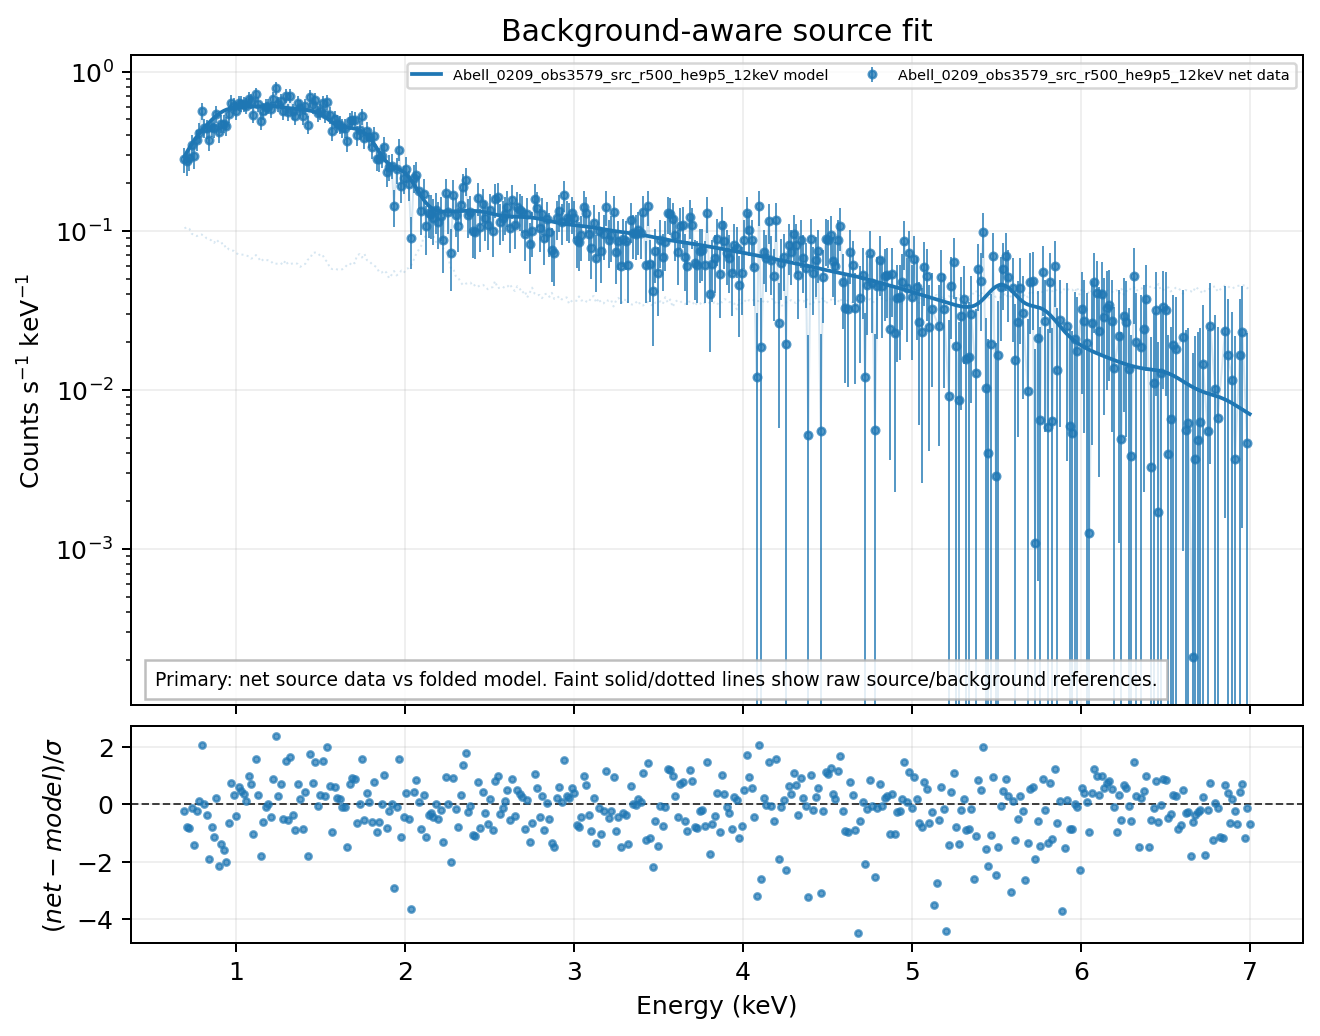
\includegraphics[width=0.95\linewidth]{output/figures/spectral/Abell_0209_fit.png}
  \caption{Abell 0209 的 full-\Rfive{} 光谱 QA 图。新版图像区分 raw source/background 和 net source/model，避免早期 WSTAT 诊断图中 raw source counts 与 folded model 直接比较造成的视觉 offset。}
  \label{fig:spectral-qa}
\end{figure}

\section{标度关系拟合方法}

标度关系使用 \citet{kelly2007} 的 Bayesian linear regression 方法 \texttt{linmix}。拟合采用以 10 为底的对数，考虑双轴测量误差，并报告固定自变量下因变量方向的内禀散布（dex）。模型形式为
\begin{equation}
  \log_{10}\left[\frac{Y}{E(z)^{\gamma}}\right]
  = \alpha + \beta \log_{10}\left(\frac{X}{X_{\mathrm{piv}}}\right).
\end{equation}
具体关系为
\begin{align}
  E(z)^{-2} L_{\mathrm{X,bol}} &= A \left(\frac{M_{500}}{3\times10^{14}M_\odot}\right)^\beta,\\
  E(z)^{-2/3} T_{\mathrm{X}} &= A \left(\frac{M_{500}}{3\times10^{14}M_\odot}\right)^\beta,\\
  E(z)^{-1} L_{\mathrm{X,bol}} &= A \left(\frac{T_{\mathrm{X}}}{5\,\mathrm{keV}}\right)^\beta.
\end{align}
红移演化指数固定为自相似对比值。这里的 pivot 主要定义归一化 $A$ 的报告位置，而不是决定斜率本身；如果一致地改变 pivot，截距会变换，但物理直线、内禀散布和斜率原则上不应改变。由于当前保留样本的质量大多高于 $3\times10^{14}M_\odot$，未来如果重点讨论 normalization，可以在服务器上额外给出以样本中心为 pivot 的版本；本文主线仍聚焦斜率和散布。质量误差来自 canonical products 中记录的弱透镜文献误差。\Rfive{} 误差由 \Mfive{} 误差传播得到，只作为孔径来源记录，不作为独立的 \texttt{linmix} 误差项。

\section{结果}

\subsection{Full-\texorpdfstring{$R_{500}$}{R500} 基线结果}

Full-\Rfive{} 主样本包含 18 个星系团。图~\ref{fig:full-scaling} 展示三个基线关系。\Lx--\Mfive{} 的斜率为 $\beta=1.08^{+0.45}_{-0.48}$，内禀散布为 0.169 dex；在当前误差下与自相似斜率 $4/3$ 一致。\Tx--\Mfive{} 的斜率为 $\beta=0.50^{+0.29}_{-0.27}$，内禀散布为 0.117 dex，略低于但仍与自相似值 $2/3$ 相容。\Lx--\Tx{} 的斜率为 $\beta=0.77^{+0.47}_{-0.44}$，内禀散布为 0.227 dex，是三个关系中最不稳定、噪声最大的一个，也明显浅于常见 Chandra 文献结果 \citep{maughan2012}。

\begin{figure}[p]
  \centering
  \begin{subfigure}{0.48\linewidth}
    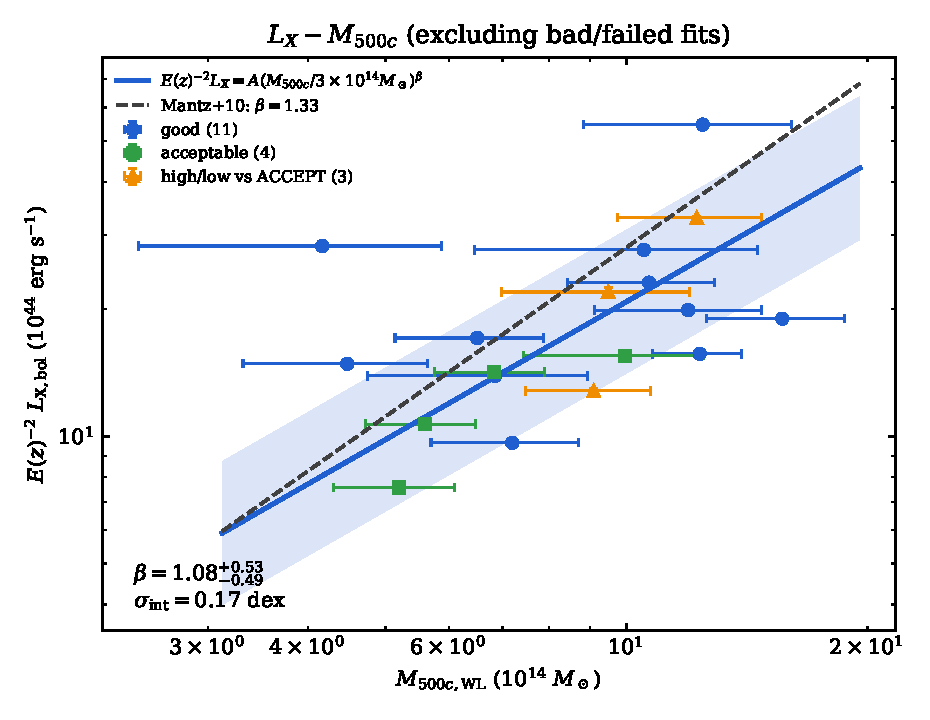
\includegraphics[width=\linewidth]{output/figures/scaling/lx_m500_linmix_exclude_bad.pdf}
    \caption{\Lx--\Mfive}
  \end{subfigure}
  \begin{subfigure}{0.48\linewidth}
    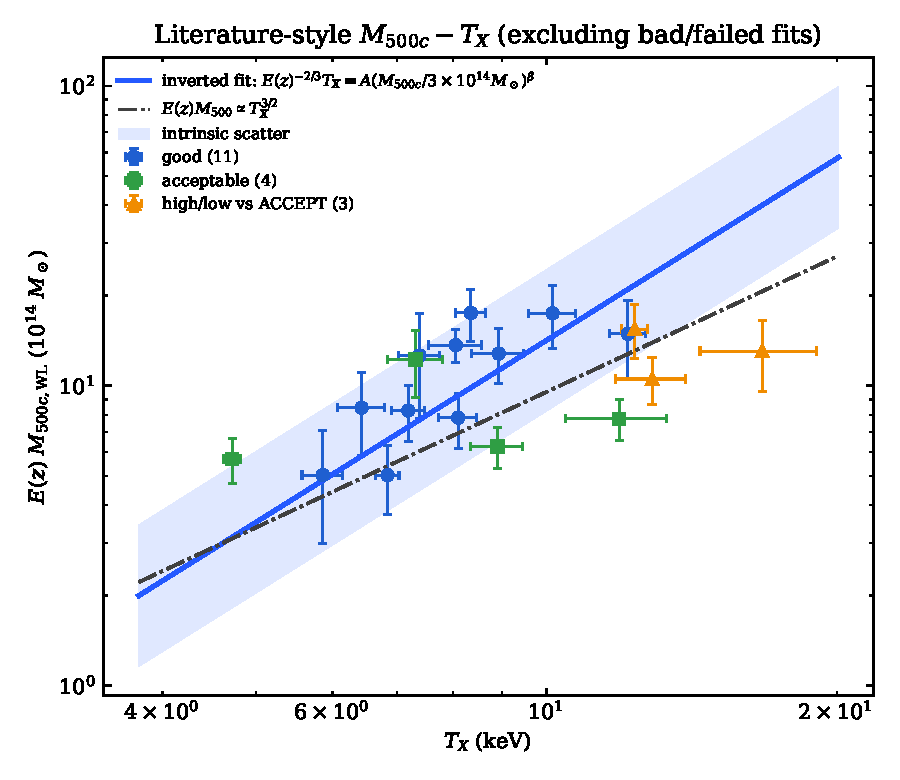
\includegraphics[width=\linewidth]{output/figures/scaling/m500_tx_literature_style_exclude_bad.pdf}
    \caption{\Tx--\Mfive}
  \end{subfigure}
  \begin{subfigure}{0.58\linewidth}
    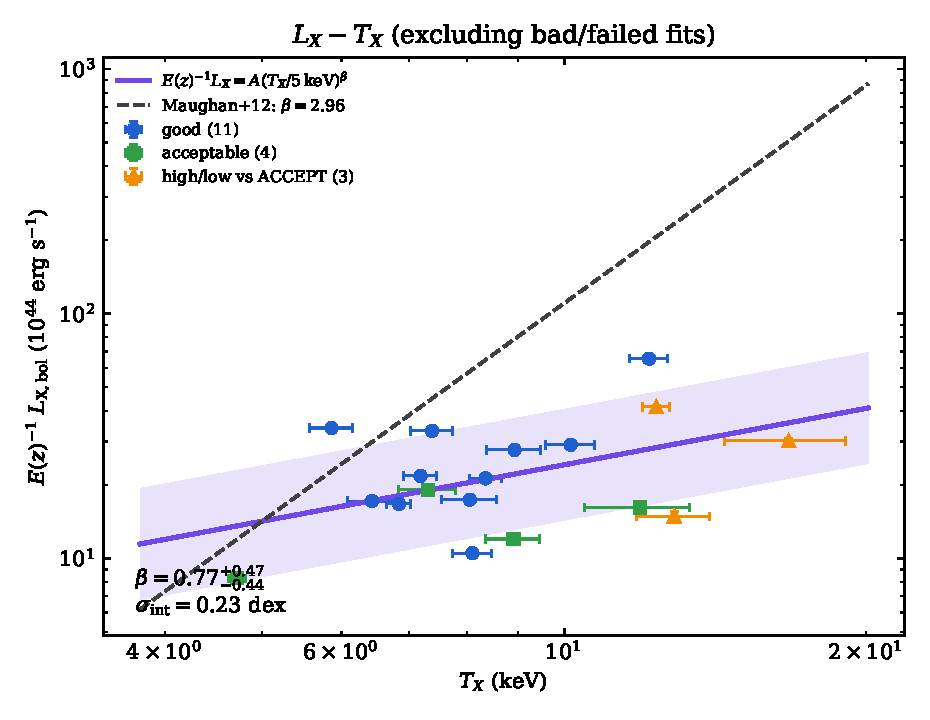
\includegraphics[width=\linewidth]{output/figures/scaling/lx_tx_linmix_exclude_bad.pdf}
    \caption{\Lx--\Tx}
  \end{subfigure}
  \caption{18 个星系团 \texttt{exclude\_bad} 样本的 full-\Rfive{} 基线标度关系。}
  \label{fig:full-scaling}
\end{figure}

\subsection{Core-excised 对比}

Core-excised 分支对同一 18 个星系团使用 $0.15$--$1.0\Rfive$ 孔径。图~\ref{fig:core-scaling} 展示对应结果。\Lx--\Mfive{} 斜率为 $\beta=1.15^{+0.54}_{-0.51}$，散布 0.186 dex；\Tx--\Mfive{} 斜率为 $\beta=0.55^{+0.36}_{-0.34}$，散布 0.157 dex；\Lx--\Tx{} 斜率为 $\beta=0.69^{+0.40}_{-0.41}$，散布 0.245 dex。Core-excised 与 full-\Rfive{} 的质量标度关系斜率在统计误差内一致。对这个小而异质的样本，core excision 并没有降低测得的散布；合理原因包括样本量小、Chandra 曝光不均匀、仍保留若干高温系统，以及 core-excised \Tx{} 当前使用 10\% 误差 fallback。

\begin{figure}[p]
  \centering
  \begin{subfigure}{0.48\linewidth}
    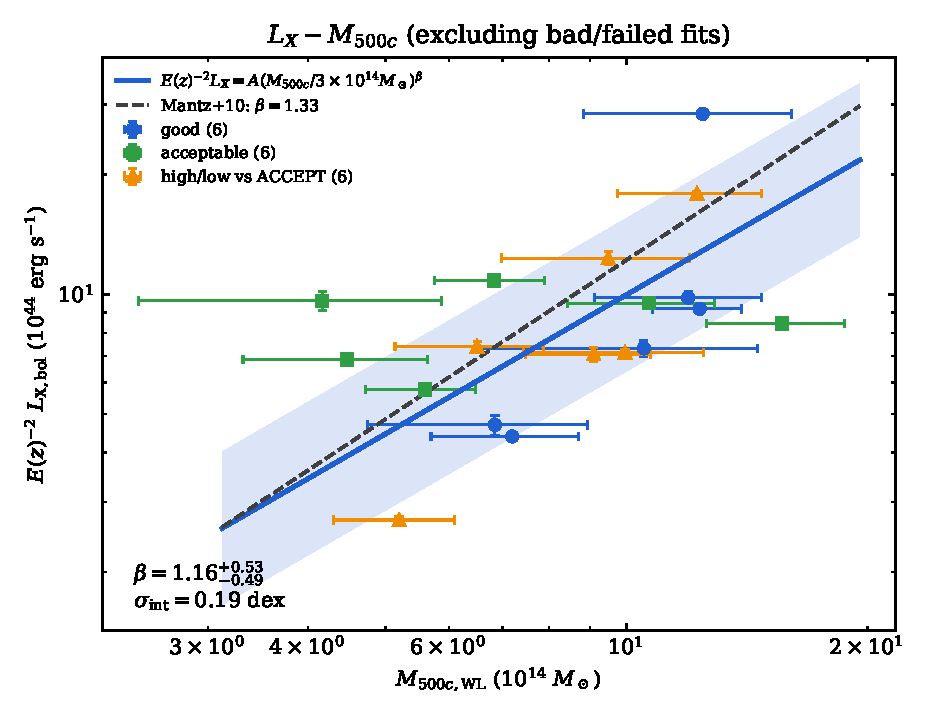
\includegraphics[width=\linewidth]{output/figures/scaling/core_excised/lx_m500_linmix_exclude_bad.pdf}
    \caption{\Lx--\Mfive}
  \end{subfigure}
  \begin{subfigure}{0.48\linewidth}
    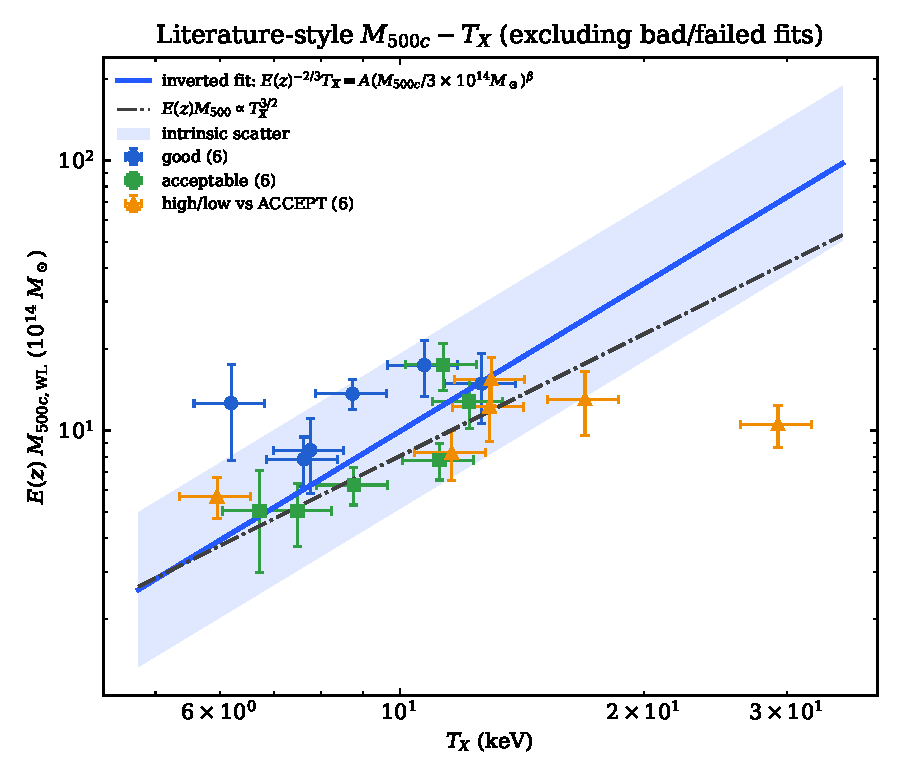
\includegraphics[width=\linewidth]{output/figures/scaling/core_excised/m500_tx_literature_style_exclude_bad.pdf}
    \caption{\Tx--\Mfive}
  \end{subfigure}
  \begin{subfigure}{0.58\linewidth}
    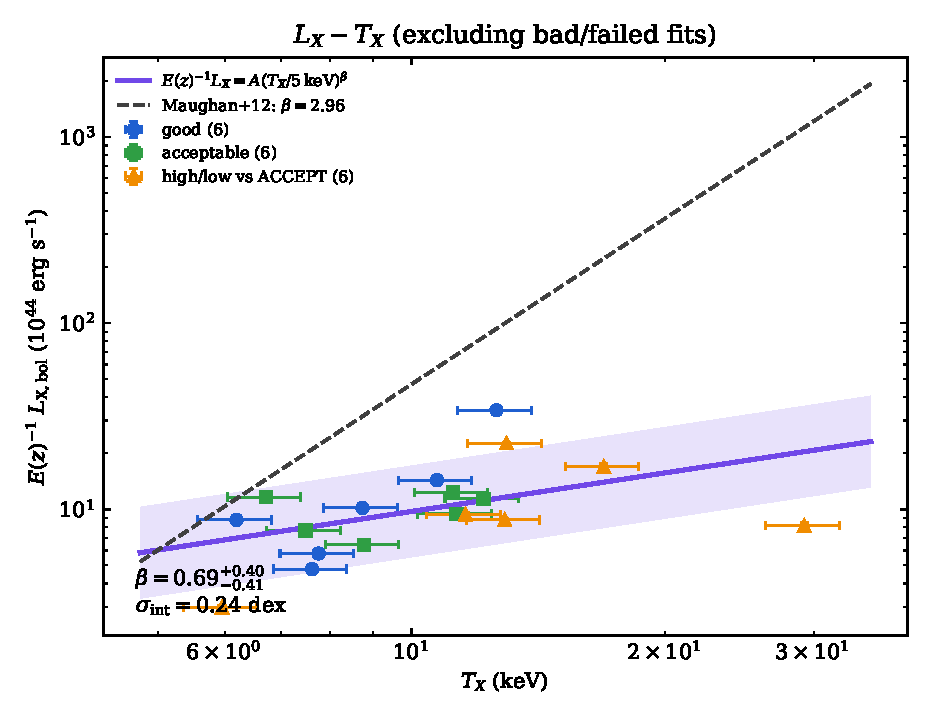
\includegraphics[width=\linewidth]{output/figures/scaling/core_excised/lx_tx_linmix_exclude_bad.pdf}
    \caption{\Lx--\Tx}
  \end{subfigure}
  \caption{同一 18 个星系团样本的 core-excised $0.15$--$1.0\Rfive$ 标度关系。}
  \label{fig:core-scaling}
\end{figure}

\begin{table}[t]
\centering
\caption{\texttt{exclude\_bad} 主样本标度关系结果。}
\label{tab:scaling}
\begin{tabular}{llcccc}
\toprule
孔径 & 关系 & $N$ & $\beta$ & 内禀散布 & 注释 \\
 & & & & (dex) & \\
\midrule
Full \Rfive{} & \Lx--\Mfive{} & 18 & $1.08^{+0.45}_{-0.48}$ & 0.169 & 基线 \\
Full \Rfive{} & \Tx--\Mfive{} & 18 & $0.50^{+0.29}_{-0.27}$ & 0.117 & 基线 \\
Full \Rfive{} & \Lx--\Tx{} & 18 & $0.77^{+0.47}_{-0.44}$ & 0.227 & 最不稳定 \\
$0.15$--$1.0\Rfive$ & \Lx--\Mfive{} & 18 & $1.15^{+0.54}_{-0.51}$ & 0.186 & Core-excised \\
$0.15$--$1.0\Rfive$ & \Tx--\Mfive{} & 18 & $0.55^{+0.36}_{-0.34}$ & 0.157 & Core \Tx{} 使用 10\% fallback \\
$0.15$--$1.0\Rfive$ & \Lx--\Tx{} & 18 & $0.69^{+0.40}_{-0.41}$ & 0.245 & Core \Tx{} 使用 10\% fallback \\
\bottomrule
\end{tabular}
\end{table}

\subsection{质量控制与敏感性检验}

被排除的 5 个系统是质量控制失败对象，而不是未探测对象。Abell 0697 和 MS2137--2353 给出极端温度和很差的拟合行为；Abell 0750 早期数据拟合质量差；RXJ1347.5--1145 在纳入全部 ObsID 后结果变差；ZwCl 0857.9+2107 与 ACCEPT 参考值/孔径比较不一致。若将这些对象放入主回归，结果会主要反映失败光谱，而不是星系团标度关系。

保留的 high/suspect 系统通过 leave-one-out 重新拟合检验。逐个移除 Abell 0068、Abell 0611、MACSJ0647.7+7015 或 MACSJ1206.2--0847 后，\Lx--\Mfive{} 和 \Tx--\Mfive{} 的斜率变化都小于当前统计误差。\Lx--\Tx{} 对 Abell 0611 和 MACSJ1206.2--0847 更敏感，因此更适合作一致性检查，而不是主科学结论。

\section{讨论}

Full-\Rfive{} 与 core-excised 的质量标度关系斜率在当前误差内一致。这说明主质量标定并非完全由 cool-core 发射驱动。另一方面，core excision 没有降低散布，这与一些更大、更均匀的文献样本不同 \citep{pratt2009,mantz2010,mantz2016}。这一点不应过度解释：本项目主样本只有 18 个星系团，CLASH 与 LoCuSS 选择函数不同，Chandra 观测深度不均匀，还包含若干高温保留系统，并且 core-excised \Tx{} 误差仍有 fallback。

与文献比较，\Tx--\Mfive{} 斜率大体符合自相似图像，也支持温度作为较低散布质量 proxy 的经验认识。\Lx--\Mfive{} 斜率低于一些陡的光度--质量测量，但在大误差下仍与自相似值相容。\Lx--\Tx{} 斜率偏浅且不稳定，可能来自温度离群点、小动态范围和测量协方差。若要发展到发表级分析，需要进一步强化背景 QA、补齐 confidence interval，并在扩展样本后考虑带选择函数的层级模型。

\section{结论}

\begin{enumerate}
\item 本项目完成了从 Chandra 数据到标度关系的完整流程：CIAO 重新处理、点源 masking、逐 ObsID 光谱、Sherpa WSTAT 拟合、canonical 光谱表和 \texttt{linmix} 回归。
\item 最终主样本包含 18 个具有弱透镜质量的 CLASH+LoCuSS 星系团；5 个 bad/failed 光谱对象从主拟合中排除。
\item Full-\Rfive{} 基线结果为 $\beta_{\Lx-M}=1.08^{+0.45}_{-0.48}$、$\beta_{\Tx-M}=0.50^{+0.29}_{-0.27}$，内禀散布分别为 0.169 dex 和 0.117 dex。
\item Core-excised 分支给出一致的质量标度关系斜率，因此当前结论对 core excision 稳健。
\item \Lx--\Tx{} 关系最浅、噪声最大，应作为敏感性受限的一致性检查，而不是主结果。
\end{enumerate}

\appendix
\section{20 分钟口头报告提纲}

这份报告可以作为上台前的讲稿参考。报告时不需要逐段照读，重点是保持“物理链条”和“项目流程”清晰。

\begin{table}[ht]
\centering
\caption{建议的 20 分钟报告结构。}
\begin{tabular}{p{0.13\linewidth}p{0.25\linewidth}p{0.52\linewidth}}
\toprule
时间 & 部分 & 主要讲述重点 \\
\midrule
2 min & 动机 & 星系团同时连接宇宙学和重子物理；X 射线热气体可以追踪质量，是因为它被束缚在星系团引力势阱中。 \\
4 min & 物理标度逻辑 & 按图~\ref{fig:physical-chain} 讲：\Mfive{} 决定势阱深度，势阱决定 \Tx{} 和气体密度，气体产生 \Lx{}，真实星系团带来内禀散布。 \\
4 min & 样本和 Chandra 流程 & 说明 CLASH+LoCuSS 样本、23 个完成处理的星系团、18 个主样本，以及为什么光谱必须保留逐 ObsID 的响应。 \\
5 min & 光谱拟合和背景 & 强调 absorbed APEC、WSTAT、blank-sky 9.5--12 keV 重归一化、XRB 分量，以及背景控制为什么是技术风险核心。 \\
3 min & 标度关系结果 & 重点讲 full-\Rfive{} 的 \Lx--\Mfive{} 和 \Tx--\Mfive{} 斜率，再用 core-excised 分支说明结论稳定性。 \\
2 min & 局限和结论 & 总结质量标度关系斜率在误差内稳定，\Lx--\Tx{} 最不稳定；未来改进需要补齐置信区间和加强背景 QA。 \\
\bottomrule
\end{tabular}
\end{table}

最简洁的收尾句可以是：本项目说明 Chandra 测得的热气体观测量总体上能够追踪弱透镜晕质量，但当前精度受小样本、非均匀数据质量和背景敏感的光谱建模限制。

\section{保留样本光谱表}

\begin{longtable}{lrrrrrr}
\caption{18 个保留星系团样本。光度为 bolometric，单位 $10^{44}\,\mathrm{erg\,s^{-1}}$。}\\
\toprule
星系团 & $z$ & $M_{500}$ & $T_{\rm full}$ & $L_{\rm full}$ & $T_{\rm core}$ & $L_{\rm core}$ \\
 & & ($10^{14}M_\odot$) & (keV) & & (keV) & \\
\midrule
\endfirsthead
\toprule
星系团 & $z$ & $M_{500}$ & $T_{\rm full}$ & $L_{\rm full}$ & $T_{\rm core}$ & $L_{\rm core}$ \\
 & & ($10^{14}M_\odot$) & (keV) & & (keV) & \\
\midrule
\endhead
Abell 0209 & 0.206 & 12.34 & 8.05 & 19.22 & 8.74 & 11.26 \\
Abell 0068 & 0.255 & 6.83 & 11.90 & 18.34 & 11.19 & 13.99 \\
Abell 0267 & 0.230 & 5.60 & 8.90 & 13.45 & 8.77 & 7.24 \\
Abell 0383 & 0.187 & 5.20 & 4.72 & 9.09 & 5.95 & 3.25 \\
Abell 0586 & 0.171 & 7.20 & 8.10 & 11.41 & 7.62 & 5.19 \\
Abell 0611 & 0.288 & 9.10 & 12.87 & 17.18 & 29.23 & 9.47 \\
Abell 2261 & 0.224 & 15.65 & 8.35 & 23.73 & 11.30 & 10.56 \\
MACSJ0329.7--0211 & 0.450 & 6.51 & 7.19 & 27.58 & 11.58 & 11.94 \\
MACSJ0429.6--0253 & 0.399 & 6.85 & 6.43 & 21.14 & 7.75 & 7.14 \\
MACSJ0647.7+7015 & 0.584 & 9.49 & 16.74 & 41.54 & 16.90 & 23.33 \\
MACSJ0744.9+3927 & 0.686 & 11.94 & 10.15 & 42.52 & 10.72 & 20.95 \\
MACSJ1115.9+0129 & 0.352 & 10.67 & 8.92 & 33.31 & 12.17 & 13.68 \\
MACSJ1206.2--0847 & 0.440 & 12.24 & 12.35 & 52.51 & 12.96 & 28.60 \\
MACSJ1720.3+3536 & 0.391 & 9.96 & 7.32 & 23.38 & 12.89 & 10.76 \\
MACSJ1931.8--2635 & 0.352 & 10.51 & 7.39 & 39.81 & 6.20 & 10.54 \\
RXJ1532.9+3021 & 0.363 & 4.17 & 5.86 & 41.16 & 6.71 & 14.04 \\
RXJ2129.7+0005 & 0.234 & 4.48 & 6.84 & 18.76 & 7.48 & 8.67 \\
RXJ2248.7--4431 & 0.348 & 12.45 & 12.15 & 78.38 & 12.61 & 40.77 \\
\bottomrule
\end{longtable}

\bibliographystyle{plainnat}
\bibliography{references}

\end{document}
